\chapter{Information about Project}
% While writing about these phases, you should include also:  
% • problems encountered,  
% • their solutions found in the organization,  
% • methods followed,  
% • evaluation  of the project management,  
% • key points you have learned.
In this chapter, I will be explaining technical details regarding the 
project. To provide better context, I shall be introducing the project first. 
\par
PGMaster is an administration tool that mainly intends to help database and 
system administrators. PGMaster provides an interface for the systems that 
utilize containers which are homes to databases. Using Docker containers, our 
system creates and manages clusters. These clusters offer capabilities like 
high availability and data integrity. With various configurations, databases 
can be set up with modes like master, standby and more. Intended users of the 
product is admins that manage systems with high amounts of transactions. 
Whether it is private or official organization, many admins perform high level 
database management operations using tools on command-line interface (CLI). 
PGMaster can be considered as an abstraction over such interfaces as it allows 
critical operations to be initiated, observed and completed using a graphical 
user interface (GUI).
\par
PGMaster, although trivializing many tasks for admins, provides a CLI over the 
web application as well. This is achieved using WebSocket as well as various 
libraries which will be explained further in detail later on.
\par
Without any due, I will get into the phases I have been through during my 
internship.
\section{Analysis Phase}
On my first day of the internship, after being given a computer and setting up 
my development environment, I have been introduced to Derviş. Prior to my 
involvement, he was the one and only contributor of the project. It was 
determined that I was going to implement front-end application of the system. 
After discussing the high level requirements of the system, it was clear to be 
that library that I was going to use for the project, namely Reactjs, was 
suitable. The project didn't have any document prior to implementation.
\par
Before my involvement, Derviş had already implemented some of the back-end 
application modules which was using Java and Spring Boot framework. Being an 
experienced software developer (with 20+ years of experience), he was quite 
comfortable implementing Java and bash code. He also had extensive knowledge 
on PostgreSQL and database management systems in general. However, he needed 
a hand with the front-end application. There was only a JavaServer Pages (JSP) 
implementation with a form and some buttons written in HTML which were not 
sufficient for more sophisticated and dynamic nature of the system.
\par
We have discussed the project briefly and I proceeded to learn Reactjs the 
following days. I will be telling about implementation related details that 
were discussed on initial meetings on following sections. After understanding 
the general requirements of the system I have spent time analyzing the 
following:
\begin{itemize}
    \item Candidate modules and entities.
    \item Nature of the data to be processed.
    \item Design related constraints.
    \item Documentation needs.
    \item Conventions to be followed during implementation.
\end{itemize}

I will try to explain considerations I have had for each of these items. 

\subsection{Modules and Entities}

Before jumping into these items, it seems necessary to talk about PGMaster 
modules and entities. The modules can be listed as follows:

\begin{itemize}
    \item \textbf{PGManager:} Even if the name suggests something similar to 
    PGAdmin, a web-based GUI tool that is commonly used to interact with 
    PostgreSQL databases, it is actually the back-end of PGMaster application. 
    It is written in Java (using Spring Boot framework) and it has two main 
    purpose: Performing CRUD operations on pgm database, the database that 
    contains ``meta'' data regarding the application itself and manage 
    operations that affect PGMaster entities. These entities will be 
    explained below.
    \item \textbf{Grafana:} Grafana is a multi-platform open source analytics 
    and interactive visualization web application. It provides charts, 
    graphs, and alerts for the web when connected to data sources. Our 
    web application's front-end is intended to be embedded into one of 
    Grafana's custom panels. Within the context of PGMaster, this is its 
    most relevant purpose. Other than that, various services and endpoints 
    that works on the container of PGMaster provide the data Grafana shows. 
    As understood, the application PGMaster is also containerized. The 
    content of this container will also be mentioned later on the document.
    \item \textbf{WeTTY:} WeTTy (Web + TTY) is an npm module that makes it 
    possible to have terminal access in browser over HTTP(S). As mentioned 
    before, PGManager is intended to offer necessary tools that would help 
    advanced users to perform various actions on CLI. We have decided that 
    using a library for this purpose would be beneficial over implementing 
    our own module. It basically utilizes WebSocket protocol to establish 
    an SSH connection. In PGManager, we intend to offer access to PG hosts 
    and containers using this library.
    \item \textbf{PG-Web:} This is the application I have implemented from 
    the beginning using Typescript and Reactjs. It basically provides a 
    GUI to PGManager users where they can perform various actions such as 
    creating and initializing PGContainers, taking backups and restoring 
    them, monitoring clusters and their nodes' status etc. PGMaster has 
    over 100 such operations. While most of them needs only one parameter 
    to be provided, some of them require more sophisticated data to be 
    provided. For sake of simplicity, only some portions of these operations 
    will be explained on the following sections of the document.
\end{itemize}

These four modules are the main ``pillar stones'' of a PGMaster ecosystem. 
Organizations that have systems with multiple databases which needs to deal 
with high volumes of transactions while maintaining high availability and 
also security and integrity of their data may unfortunately not have admins 
that are capable of performing operations that were mentioned above trivially. 
These modules intend to offer tools that are necessary to maintain, operate 
and administrate these systems whether they have advanced database 
administration skills or not.
\par
I have mentioned that PGMaster have different entities. I will be listing 
what they are and what purpose do they serve below:
\begin{itemize}
    \item \textbf{PGContainer:} As mentioned briefly before, databases 
    within PGMaster ecosystem lives inside Docker containers. These databases 
    have different configurations depending on their cluster modes. These 
    modes can be simple listed as (I am not creating another list!) master, 
    standby and replica. Intuitively, these names indicate whether a container 
    contains the ``main'' database or its ``copies''. Depending on the status 
    of a master database (and its container), various operations can be 
    triggered using PG-Web. These containers come together and create a 
    cluster, more specifically PGCluster. It is worth mentioning that PGMaster 
    itself is a container as well. This container is intended to contain 
    modules mentioned above. While the main benefit of using a container is 
    to be able to deploy PGMaster on an organization easily, other benefits of 
    using a container could also be considered as the added advantages.
    \item \textbf{PGHost:} Naturally, a host is required to run Docker engine 
    and PGHost is the host that houses these containers. While PGHost mainly 
    indicate a dedicated, physical server, it can also be a virtual private 
    server (VPS). These hosts houses PGContainer and their availability 
    directly impacts health of a PGCluster. Naturally, a PGContainer may have 
    nodes that lives inside different PGHosts. I think for the scope of this 
    document, this should suffice explaining what a PGHost is.
    \item \textbf{PGCluster:} PGCluster, to be brief, is the combination of 
    multiple PGContainers. Its nodes (PGContainers) may or may not live inside 
    different PGHosts. Containers alone do not provide hi(gh availability and 
    clusters are utilized to provide it. PGClusters are shown with a topology 
    inside PG-Web. Entity management view, which will be explained later on,
    allows users to configure their nodes inside a PGCluster.
    \item \textbf{PGBackupServer:} As understood from the name, it is simply 
    a server that contains backup files of a PGContainer database. Backup 
    data is transferred to this entity on desired intervals and when the need 
    rises, this entity provides the data that needs to be recovered.
\end{itemize}

These four entities were the main entities that were necessary to have a 
functional PGMaster ecosystem. I have spent first two weeks creating views 
to create, update and delete show these entities. The main benefit of using 
Reactjs over regular HTML/CSS/JS stack for the GUI was to be able to render 
these entities optimally and dynamically without having to update the page. 
While Javascipt makes a regular web page dynamic to some extend, Reactjs 
allows users to manipulate data and have Document Object Model (DOM) to be 
synchronized seamingly. As stated on the official documents of Reactjs, 
Web Components and Reactjs are complementary, i.e., they solve different 
problems. While Web Components provide encapsulation of reusable components, 
Reactjs provides declarative implementation. So it is safe to say that real 
benefit of using Reactjs is felt by developers, rather than users. I don't 
mean to go out of scope of this document and explain benefits of React, so I 
will keep it brief. In PGMaster context, React allows us to utilize having 
declarative implementation, meaning the developer can set the ``rules'' for 
a view and the view updates automatically with the rules provided by the 
developer without needing to refresh the page user interacts. I have already 
mentioned that PG-Web, the module I have implemented is embedded into Grafana. 
It goes without saying that user should be able to observe the changes on 
PGMaster GUI without needing to refresh the web page, especially considering 
that Grafana already allows this for other views than PGMaster. In that sense, 
usage of a library such as Reactjs was vital during the implementation.

\subsection{Data}
The data that circulates on PGMaster could be divided into two:
\begin{itemize}
    \item \textbf{Entity Data:} PGMaster has its own database to contain 
    details regarding entities. While adding/updating/deleting these entities, 
    a PostgreSQL database (pgm) is used. PGManager (the back-end) has numerous 
    endpoints (listHosts, listContainers etc.) that feed the front-end 
    application PG-Web. Entity data is fetched to render initial view of
    PG-Web and it is updated performing various CRUD operations on the said 
    database. When a user updates entities, the change is immediately 
    reflected on PG-Web. This ensures users to have the latest updates on 
    PGMaster to be synchronized on the GUI they are using. I have implemented 
    the GUI in a way that a user can have sufficient feedback and information 
    whether operations they have initiated were successful or not.
    \item \textbf{Operation Results:} While most of the configuration a user 
    can make is intended to be performed once or twice, the operations on a 
    PGMaster entity is expected to be more repetitive. Depending on the status 
    of a PGMaster entity, these operations may fail or succeed. I have 
    implemented a view where users may see the results of the operations they 
    have initiated. We have realized that HTTP status codes wouldn't suffice 
    since they don't provide information regarding what went during the 
    execution of a PGMaster operation. Then Derviş decided that we can use 
    slightly more sophisticated response objects, namely Rx, to provide user 
    more than just a status code. These objects contain fields like error 
    code, command, result text, hint, execution time, container name, host 
    name, cluster name, path, details and more. I have implemented various 
    views that allow users to view these. I'd like to mention a detail 
    regarding the implementation of these views. When a user triggers a 
    command to execute, this command have potential to trigger other commands. 
    These commands may or may not fail depending on a lot of factors (such 
    as permissions, status of the target entity etc.) and user should be 
    able to identify when did an operation has failed with precision. I have 
    offered two different alternatives for users. Firstly, users may see 
    these commands and their results with indentation on a table. As an 
    alternative to this, users may also see a command and its ``child'' 
    commands in a tree-like view. Upon discussions with Derviş, we have decided 
    to use the first, as it would be practially impossible to show the results 
    of these commands' results on a tree view, considering Grafana can only 
    provide so much space.

\end{itemize}

\subsection{Design Constraints}

As mentioned before, PG-Web is intended to be shown among other views Grafana 
has. I must admit that I have faced the challenge of ``unknown requirements''. 
To elaborate, PGMaster is intended to be used by ``power users'' that have 
access to hardware such as 4K monitors. However, Derviş occasionally has 
tested the views on his personal mobile device and this forced me to consider 
another constraint which was being responsive. Fortunately, the library I have 
used (Semantic UI React) provided predefined solutions which allowed users to 
interact PG-Web seamingly. Prior to my internship at Siren Bilisim, I have 
considered web development rather trivial. However, I have learned that 
implementing GUIs that just work on different devices is indeed a challenge 
where you have to consider countless edge cases. I am not sure how viable the 
end product will be on different mobile devices (tablets and movile phones 
running Android or IOS) but I have spent decent amount of time on making our 
Uproduct work on different devices. Unfortunately, Siren Bilişim didn't have 
any UI/UX designer which was assigned to work on this project, so I had to 
come up with my own designs and implementations.

\subsection{Documentation}

Having had an introduction to software requirements specification (SRS) and 
software development lifecycle in general in our Software Engineering course, 
I usually try and understand the needs of any development activity prior to 
actual work. Aiming to follow the same trend here, I must admit that I was 
mildly disappointed, since although we didn't have a strict timeline to 
deliver the proof of concept (PoC) version of the application, the project 
was solely maintained and developed by one person. This should have 
-expectedly- obscured the need for any form of documentation.
\par I have actively communicated with my supervisor (Koray) and colleague 
(Derviş) on the subject and I was given permission (and responsibility) to 
write SRS for the project. I did not start writing the document right away, 
because it took me a while to fully grasp the overall needs and constraints 
of the system and the rest ofthe requirements naturally needs further 
discussion with stakeholders and the potential users. I still had chance to 
write some of the document by myself and it will be attached to the report. 
Final version of the SRS is expected to be completed after it is presented 
to The Ministry of Health.

\subsection{Conventions}

Reactjs, the library that I have used extensively during the implementation 
of PG-Web is a libarary that was open-sourced in 2013. Since that time, 
with the help of community (that consists of developers from all around the 
world) Facebook switched from class-based components (and its implemenation) 
to function-based components. For sake of not getting into too much details, 
I will skip how it happened, but I adopted the function-based component 
implementation approach. With the additions of ``hooks'', Reactjs eliminated 
the need for most of the boilerplate code and I made use of this approach.

\section{Design Phase}
As explained on prior sections of the document, user interface-wise, the 
design was mostly determined on-th-go, that is, I have created the views 
using Semantic UI React and depending on the feedback I have received from 
my colleague Derviş.
\par
When it comes to system design, I have adopted the design that was initially 
proposed and partially implemented by Derviş. Our application, although 
mainly relays on operating system level operations which were invoked by 
back-end application PGManager, is an MVC application in its essence. 
Using RESTful API to manage network requests, I have took part in 
development of back-end code in order to comply with the standards better.
\par
It goes without saying that the actual layout the source code of the 
front-end and back-end applications are also relevant. This project, 
although having financial concerns and economic value, is also intended 
to be an open-source project in the long run. Having that in mind, I have 
tried to refactor the code base once I have reached certain milestones. 
For example, the source code for various React components would be on the 
same file, sometimes with poor readibility. Since the company had limited 
man power when it comes to Reactjs, I have joined communities like Reactiflux 
and communicated with different developers around the world. This community 
actively communicates on their Discord server. The server has different 
channels where people ask and answer questions ranging from high-level to 
specific errors and issues with a React application. On my third week of the 
internship, I have posted on ``code-review'' channel and I was fortunate 
enough to receive feedback from a more experienced developer. Upon his 
feedback, I refactored about 40\% of the codebase. To provide my development 
activities briefly without giving too much details, I will be sharing the 
commit history on appendices. Considering the project hierarchy is more 
relevant to the \textit{design} the latest version of the project 
(PG-Web, to be specific) can be seen above on Figure \ref{fig:files}:

\begin{figure}
    \centering
    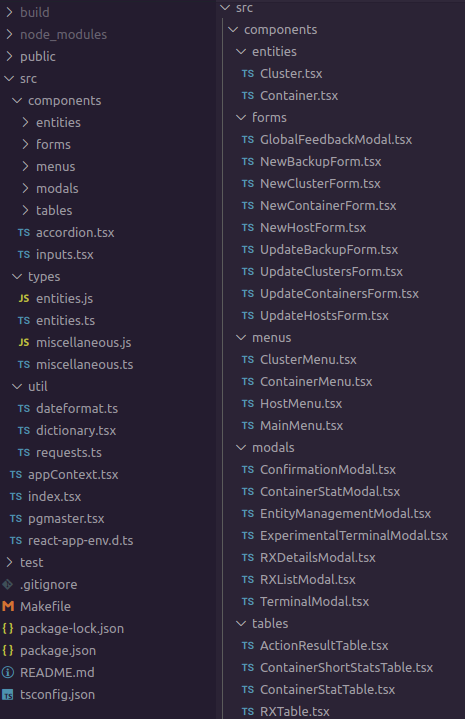
\includegraphics[width=8cm]{files.png}
    \caption{File structure of PG-Web}
    \label{fig:files}
\end{figure}

\par
As mentioned before, PGMaster has its own database pgm to save entity 
related data. This database consists of four tables, pg_container, pg_host,
pg_cluster and pg_backup. These table have their records updated with two 
main constaint. Regular SQL-related constraints and their dependency on 
the success of the operations that relates to them. In other words, when a 
user triggers a PGMaster operation from the GUI, it causes PGManager to 
execute various projects. While some of them utilize docker engine to 
start/stop/restart containers, some of them perform more sophisticated 
operations such as performing a HotStream Replica (with Delta Store), Wal 
Replica (with Delta Store), Diff backup (delta last full backup) etc. This 
database has a pretty straightforward schema which can be view on Figure 
\ref{fig:schema} below:

\begin{figure}
    \centering
    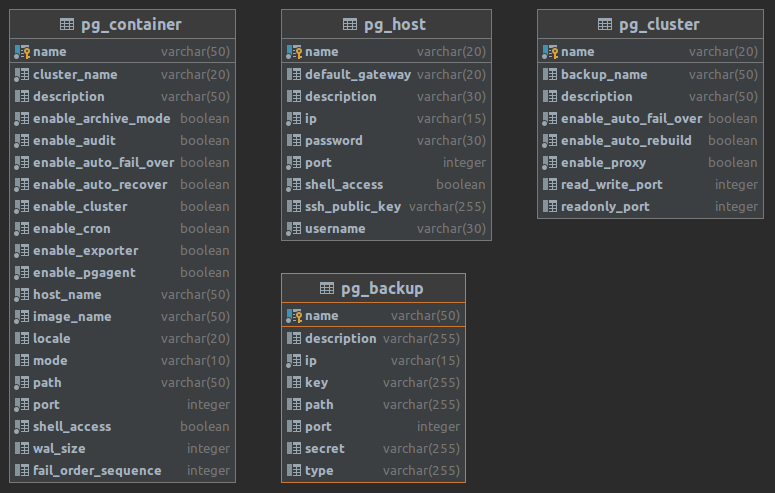
\includegraphics[width=14cm]{pgm.png}
    \caption{DB Schema of PGManager}
    \label{fig:schema}
\end{figure}

\section{Implementation Phase}
\subsection{Front-End Implementation}
I had mentioned that I had prior front-end web development using HTML, CSS and 
Javascript. However, I didn't know Reactjs and I've spent approximately one 
week getting familiar with the library. Reactjs is a Javascript library 
that was priorly used by Facebook internally and later open-sourced around 
2013. Since then the library have adopted different standards with the help 
of the community. I usually prefer sticking to official documents when I 
am learing a new technology. I have spent trying to understand what does 
Reactjs offers and what were the reasonings behind the changes that were 
added to it over the years. The main change that was implemented to the 
library was the addition of hooks. To be brief, initially Reactjs used 
class based components where you implemented a class with props and states, 
then adding bunch of bindings and other boilerplate code. From a developer's 
perspective of view, this was cumbersome. Recent versions of Reactjs 
encourage usage of hooks. Some of them are useState, useEffect, useContext,
useMemo, useCallback and more. The library allows addition of custom hooks 
which modify the state of components that are widely used in Reactjs 
applications.
\par
The main challenge I have faced learning and implementing Reactjs was that 
my prior experience with front-end web development involved writing source 
code that were mostly imperative and some functional paradigm. Reactjs, 
however, in addition to these, introduces wide usage of declarative paradigm 
where developer provides the rules for a component and the component renders 
desired views respecting the rules provided by the developer. Most of the 
optimization is provided by the library out-of-the-box which saves a lot of 
unnecessary renders. With effective usage of proper hooks and determining 
props and states carefully also yields a responsive, fast view. As mentioned 
above, PGMaster is no less active when it comes to flow of data and it is 
easily comparable to modern social media web applications such as Facebook. 
Just like a user may modify the view of, say, chat box. Similarly, PGMaster 
is expected to render PGContainers and other relevant entities with their own 
Reactjs components considering their current status. The data that determines 
which entities and their respective React components to be rendered is 
synchronized with the data that is fed by PGManager, allowing users to see 
the results of their actions and their effects which is further determined 
by the operating system and Docker Engine.
\par
I have made the mistake of refreshing the view using setInterval method of 
Javascript on my initial iterations which was conceptually against the way 
Reactjs is suppsoed to work. PG-Web is expected to trigger re-render without 
having to fetch the data that were updated by a user form, for example. To 
overcome this problem, I have learned about application-wide state solutions. 
One of the most common solutions the community offers was Redux, but I didn't 
want to use it for sake of simplicity and avoid going through the steep 
learning curve of the library. It turns out the main contributors of Reactjs 
were also aware of the issue at hand when it comes to store complicated data 
and they came up with ``context''. They added it with its own hook (in React 
16) which enabled developers to set initial data, update it using various 
sources (user input or from a new work source) and make this data available 
to React components. The main benefit of using this feature comes from the 
elimination of prop drilling. Prop drilling is the method that were widely 
used prior to context would require developer to pass data from all the way 
down to the child components from the root component and that would be 
problematic especially when the source code needed refactoring. Reactjs 
provides a strong hierarchical component structure with the help of its 
composition capabilities.
\par
As mentioned on prior sections, I have had the following data:
\begin{itemize}
    \item Clusters
    \item Hosts
    \item Containers
    \item BackupServers
\end{itemize}
Although this data doesn't look too complex, I have noticed that every change 
in these entities' respective data structures, it would trigger a re-render 
on all the application. After reading Kent C. Dodds fantastic articles 
about \href{https://kentcdodds.com/blog/application-state-management-with-react}
{Application State Management with React} and 
\href{https://kentcdodds.com/blog/how-to-use-react-context-effectively}
{How to use React Context effectively}. I came to realize that I was being too 
eager to use the new feature without making sure it was the best solution. 
When it comes to simple data such as ``darkMode'' which requires nothing but 
a boolean variable, React's Context really shines. As known, in today's web 
and mobile applications the option to have a dark/light mode is quite common. 
In such use cases, the application needs to spread this data to a lot of nodes 
in its component tree. In such cases, a toggle that changes this variable 
needs to be reflected on all the components and trigger a re-render.
\par
Long story short, I have realized that I can just use prop drilling to spread 
my entity data among components that need it. With prop drilling, there is a 
known trade-off between development time and application performance. In other 
words, although prop drilling means passing a variable from parent components 
to child components multiple times, it works seamingly with only necessary 
amount of re-renders. I ended using this for entity data while using the new 
and shiny useContext hook for the darkMode which I already implemented on 
PG-Web.
\par
Before proceeding with the rest of my implementation related activities, I'd 
like to comment a little about Typescript. Typescript is an open-source 
library that adds strongly typed language features into Javascript. This 
allows developers to avoid common pitfalls of using dynamically typed 
languages. Many of the errors that could be faced on run-time can be detected 
while ``transpiling'' with Typescript. Typescript basically transforms the 
code the developer created into a Javascript code in the end. However, it 
makes the code much safer with addition of types and interfaces. Without 
explaining too much about the language, I will share some of the types or 
interfaces I declared implementing PG-Web. These declarations allowed me to 
further utilize the capabilities of the text editor that I used by the help 
of language server, namely IntelliSense.

\begin{figure*}[b!]
    \centering
    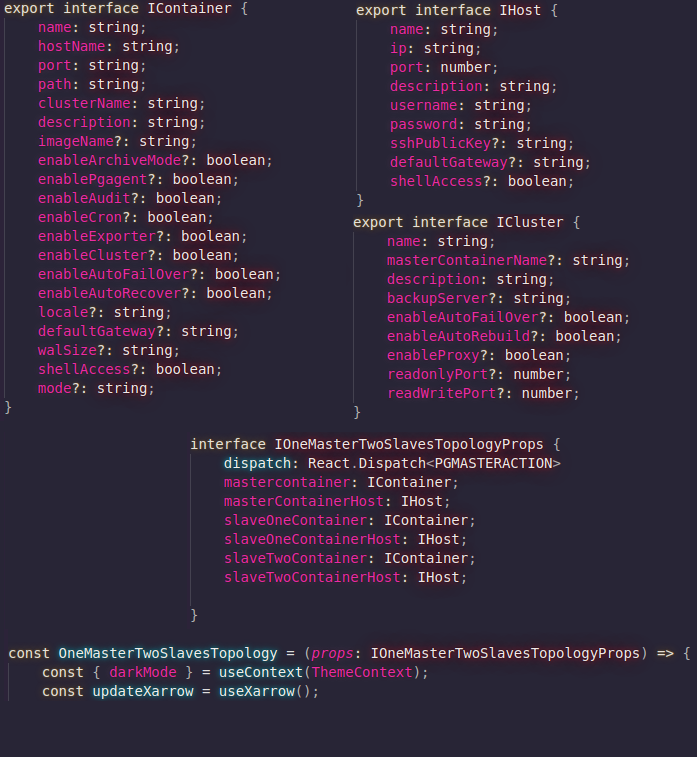
\includegraphics[width=9cm]{interfaces.png}
    \caption{Various interfaces that force type checking.}
    \label{fig:types}
\end{figure*}
\pagebreak
As seen on Figure \ref{fig:types} Typescript allows composition of basic 
primitive types. On top of the figure, interfaces (not to be confused with the 
other common usages of the word in computer science) for entities are declared.
The middle interface makes sure that proper render props are passed to the 
OneMasterTwoSlavesTopology component. And on the bottom, the common usage of 
React's useContext hook can be viewed. I have used about 40 different object 
or method interfaces throughout the development PG-Web which further improved 
the speed of debugging and testing itself.
\par
\subsection{Back-End Implementation}
Although my development activities mainly consisted of front-end development, 
following third week I felt comfortable enough with the business logic and 
participated on the development of the Java Spring Boot application. While 
sometimes work of Derviş was blocked by my implementation, there were days 
my work was blocked by his. I hopped in and modified some of the controller 
methods when needed. Furthermore, we have purchased three VPS from Contabo 
(German cloud services provider) and deployed our applications there. I have 
took active role during that process, but I'd like to tell about them on a 
separate section below. The reason I mentioned it here is that, we have 
encountered -supposedly- CORS errors while deploying. Prior to cloud 
deployment, Java and React application were running on localhost, eliminating 
most of the security related concerns. However, after deploying on publicly 
available server, we have had issues where relevant configuration were needed. 
For that, I have refactored source code on Java where security configuration 
was being implemented. It was basically setting allowed origins and allowed 
REST methods (such as GET, POST, DELETE). While editing that code, I also 
edited some of the controller methods to better comply with RESTful API 
conventions. For example, the source code for deleting entities were using 
GET methods, I changed them into DELETE methods and changed the status code 
it would return on different cases. I have also had chance to refresh my 
memory on the term ``idempotency''.
\par
Other than changing controller and security configuration source code, I have 
updated some of the testing codes. Since it is much harder to initialize 
databases with the entity data we need for testing, we utilized Java for that. 
We had data initializer tests. These also acted as migration tools when we 
needed to update our entity schemas. When Derviş pushed a commit to back-end 
application and asked me to pull changes, I would simply drop my tables and 
run data initializers. This would add the necessary data to development 
database we used. Then I was able to run my react application and I would 
have the updated fields provided by back-end API. It goes without saying that 
I used various tools (RESTED the Firefox addon, Postman, even curl) to test 
PGManager's endpoints. We have tried to enable Swagger to trivialize API 
documentation and testing processes, however it took too much time to set up 
and due to limited time we had before demo, we skipped it.
\subsection{DevOps Work}
Working with Docker containers and developing on Linux machines, it was 
inevitable to not get into DevOps related work in Siren. As I mentioned before 
to have a more realistic environment during development, we deployed our 
applications on cloud. I was able to run both PG-Web and PGManager locally, 
most of the operations PGMaster offers runs Docker engine and executes 
various commands that require extensive configuration. For that reason, I 
had to develop front-end application with ``dummy'' responses from the 
controller on back-end. Once we deployed on the server, I was able to receive 
more realistic responses, namely RX objects. These objects contained more 
details regarding the fate of an operation.
\par
While deploying our applications, another point where I hit the wall was 
to configure Nginx. We used Nginx to utilize reverse proxy. As I have listed 
above, we have 4 different modules, all running a different processes on 
different ports. I chose the path of static hosting for the web application 
which left me with three applications to set up on Nginx.
\section{Testing Phase}